% Options for packages loaded elsewhere
\PassOptionsToPackage{unicode}{hyperref}
\PassOptionsToPackage{hyphens}{url}
%
\documentclass[
]{book}
\usepackage{amsmath,amssymb}
\usepackage{iftex}
\ifPDFTeX
  \usepackage[T1]{fontenc}
  \usepackage[utf8]{inputenc}
  \usepackage{textcomp} % provide euro and other symbols
\else % if luatex or xetex
  \usepackage{unicode-math} % this also loads fontspec
  \defaultfontfeatures{Scale=MatchLowercase}
  \defaultfontfeatures[\rmfamily]{Ligatures=TeX,Scale=1}
\fi
\usepackage{lmodern}
\ifPDFTeX\else
  % xetex/luatex font selection
\fi
% Use upquote if available, for straight quotes in verbatim environments
\IfFileExists{upquote.sty}{\usepackage{upquote}}{}
\IfFileExists{microtype.sty}{% use microtype if available
  \usepackage[]{microtype}
  \UseMicrotypeSet[protrusion]{basicmath} % disable protrusion for tt fonts
}{}
\makeatletter
\@ifundefined{KOMAClassName}{% if non-KOMA class
  \IfFileExists{parskip.sty}{%
    \usepackage{parskip}
  }{% else
    \setlength{\parindent}{0pt}
    \setlength{\parskip}{6pt plus 2pt minus 1pt}}
}{% if KOMA class
  \KOMAoptions{parskip=half}}
\makeatother
\usepackage{xcolor}
\usepackage{longtable,booktabs,array}
\usepackage{calc} % for calculating minipage widths
% Correct order of tables after \paragraph or \subparagraph
\usepackage{etoolbox}
\makeatletter
\patchcmd\longtable{\par}{\if@noskipsec\mbox{}\fi\par}{}{}
\makeatother
% Allow footnotes in longtable head/foot
\IfFileExists{footnotehyper.sty}{\usepackage{footnotehyper}}{\usepackage{footnote}}
\makesavenoteenv{longtable}
\usepackage{graphicx}
\makeatletter
\def\maxwidth{\ifdim\Gin@nat@width>\linewidth\linewidth\else\Gin@nat@width\fi}
\def\maxheight{\ifdim\Gin@nat@height>\textheight\textheight\else\Gin@nat@height\fi}
\makeatother
% Scale images if necessary, so that they will not overflow the page
% margins by default, and it is still possible to overwrite the defaults
% using explicit options in \includegraphics[width, height, ...]{}
\setkeys{Gin}{width=\maxwidth,height=\maxheight,keepaspectratio}
% Set default figure placement to htbp
\makeatletter
\def\fps@figure{htbp}
\makeatother
\setlength{\emergencystretch}{3em} % prevent overfull lines
\providecommand{\tightlist}{%
  \setlength{\itemsep}{0pt}\setlength{\parskip}{0pt}}
\setcounter{secnumdepth}{5}
\usepackage{booktabs}
\usepackage{amsthm}
\makeatletter
\def\thm@space@setup{%
  \thm@preskip=8pt plus 2pt minus 4pt
  \thm@postskip=\thm@preskip
}
\makeatother
\ifLuaTeX
  \usepackage{selnolig}  % disable illegal ligatures
\fi
\usepackage[]{natbib}
\bibliographystyle{apalike}
\usepackage{bookmark}
\IfFileExists{xurl.sty}{\usepackage{xurl}}{} % add URL line breaks if available
\urlstyle{same}
\hypersetup{
  pdftitle={Modelling scenarios for nutrient-sensitive fisheries management},
  pdfauthor={Lorenzo Longobardi},
  hidelinks,
  pdfcreator={LaTeX via pandoc}}

\title{Modelling scenarios for nutrient-sensitive fisheries management}
\author{Lorenzo Longobardi}
\date{Last update: 2024-12-09}

\begin{document}
\maketitle

{
\setcounter{tocdepth}{1}
\tableofcontents
}
\chapter{Content}\label{content}

This book contains analyses and reports of the paper `\textbf{\emph{Modelling scenarios for nutrient-sensitive fisheries management}}'.

All data and code to generate the analyses are in organised in \url{https://github.com/WorldFishCenter/timor.nutrients}.

\chapter{Highlight statistics}\label{highlight}

\section{Timor-Est SSF nutritional scenario}\label{timor-est-ssf-nutritional-scenario}

\begin{figure}
\centering
\includegraphics{Timor-nutrient-sensitive-fisheries-management_files/figure-latex/unnamed-chunk-2-1.pdf}
\caption{\label{fig:unnamed-chunk-2}To define}
\end{figure}

\chapter{Nutrients distribution}\label{distribution}

\section{Fish groups}\label{fish-groups}

\begin{figure}
\centering
\includegraphics{Timor-nutrient-sensitive-fisheries-management_files/figure-latex/unnamed-chunk-3-1.pdf}
\caption{\label{fig:unnamed-chunk-3}To define}
\end{figure}

\section{Habitat and gear type}\label{habitat-and-gear-type}

\includegraphics{Timor-nutrient-sensitive-fisheries-management_files/figure-latex/unnamed-chunk-4-1.pdf}

\section{Nutritional contribution and economic profiling}\label{nutritional-contribution-and-economic-profiling}

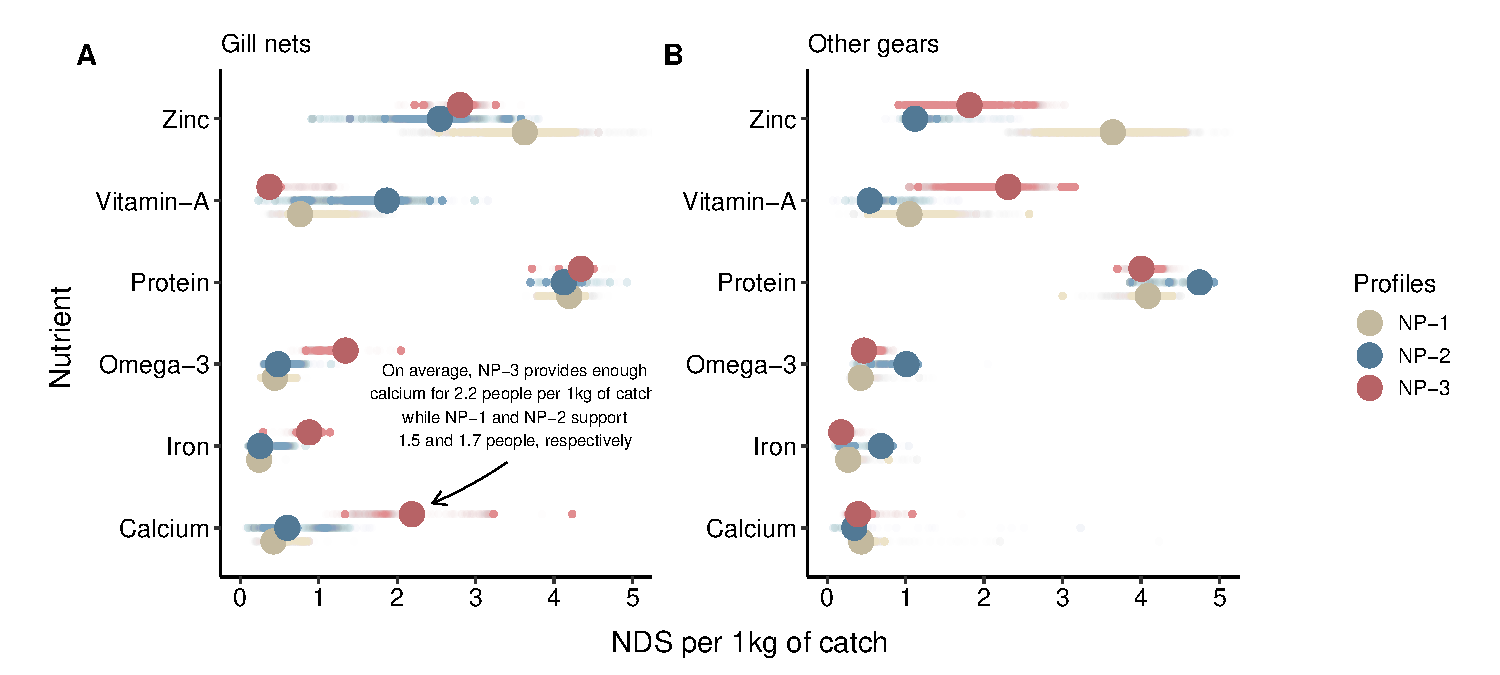
\includegraphics{Timor-nutrient-sensitive-fisheries-management_files/figure-latex/unnamed-chunk-5-1.pdf}

\chapter{Timor SSF nutritional profiles}\label{profiles}

\section{Methods}\label{methods}

\begin{verbatim}
## Warning in get_plot_component(plot, "guide-box"): Multiple components found; returning the
## first one. To return all, use `return_all = TRUE`.
\end{verbatim}

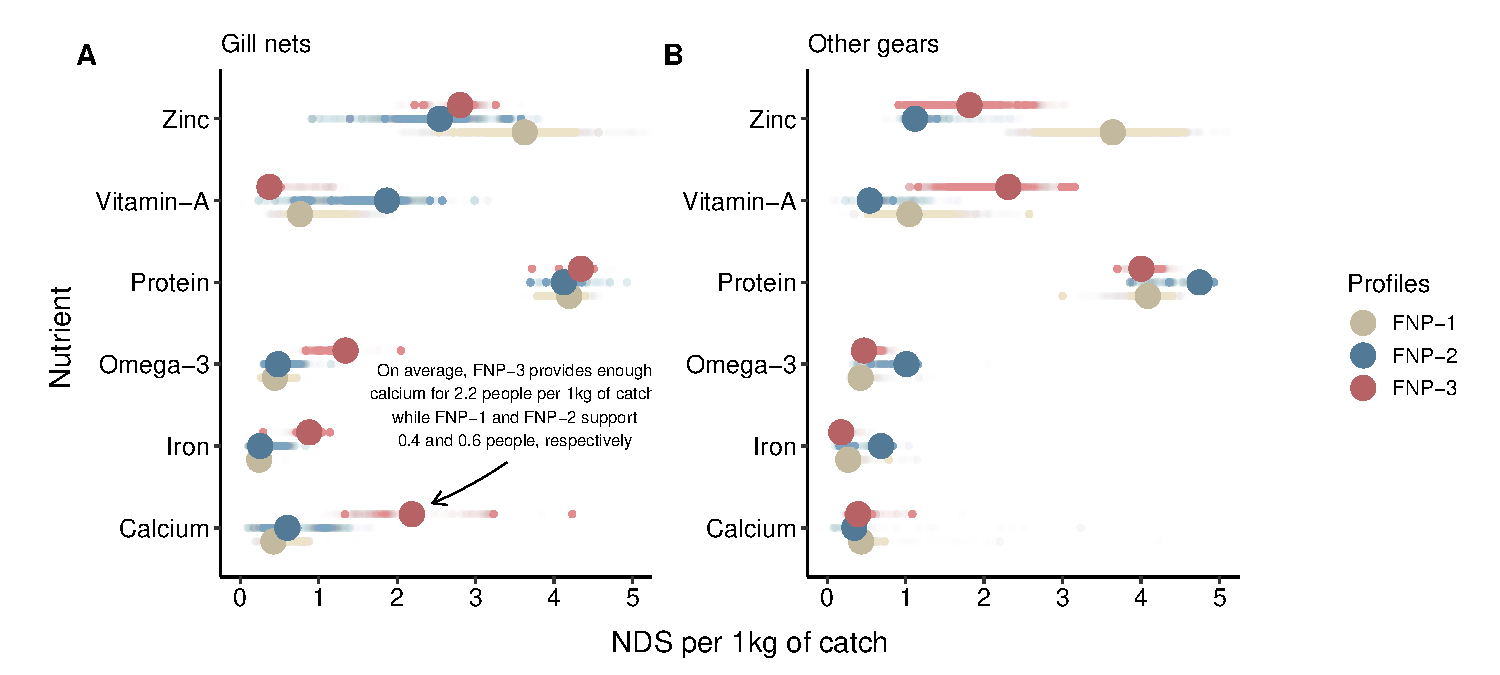
\includegraphics{Timor-nutrient-sensitive-fisheries-management_files/figure-latex/unnamed-chunk-7-1.pdf}

\includegraphics{Timor-nutrient-sensitive-fisheries-management_files/figure-latex/unnamed-chunk-8-1.pdf}

\includegraphics{Timor-nutrient-sensitive-fisheries-management_files/figure-latex/unnamed-chunk-9-1.pdf}

\subsection{XGBoost model performance}\label{xgboost-model-performance}

\includegraphics{Timor-nutrient-sensitive-fisheries-management_files/figure-latex/model-settings-1.pdf}

\includegraphics{Timor-nutrient-sensitive-fisheries-management_files/figure-latex/unnamed-chunk-10-1.pdf}

\subsubsection{Models explanation}\label{models-explanation}

\includegraphics{Timor-nutrient-sensitive-fisheries-management_files/figure-latex/unnamed-chunk-11-1.pdf}

\includegraphics{Timor-nutrient-sensitive-fisheries-management_files/figure-latex/unnamed-chunk-12-1.pdf}

  \bibliography{book.bib,packages.bib}

\end{document}
